\chapter{Linear-Quadratic Control}

% 2017/03/28
\section{Towards Global Optimal Control}
Consider a discrete-time system
\begin{gather}
  x_{k+1} = F(x_k,u_k),
\end{gather}
where $x_k$ is the state at time $k$ and $u_k$ is the input at time $k$.

Let $c(x_k,u_k)\in\R$ be the cost associated with doing $u_k$ at $x_k$.

Let $u=u_0,u_1,\dots,u_{N-1}$ and assume $x_0$ is given. The total cost over $N$ steps using $u$ is
\begin{gather}
  V_N^u(x_0) = \sum_{k=0}^{N-1} c(x_k,u_k) + \Theta(x_N),
\end{gather}
where $\Theta(x_N)$ is the terminal cost.

Assume we've found the \emph{globally} minimizing $u^*$. The best path over $N$ steps is represented by the figure below.
\begin{center}
  \begin{tikzpicture}
    \node [dot] (x0) at (0,0) {};
    \node [dot] (x1) at (1,0.2) {};
    \node [dot] (x2) at (2,0.3) {};
    \node [dot] (x3) at (3,1) {};
    \node [dot] (x4) at (4,-0.5) {};
    \node [dot] (x5) at (5,0.6) {};
    \node [dot] (xN) at (6,0.4) {};

    \node [below] at (x0) {$x_0$};
    \node [below] at (x1) {$x_1$};
    \node [below] at (x2) {$x_2$};
    \node [below] at (xN) {$x_N$};

    \draw [->] (x0) to[bend left] (x1);
    \draw [->] (x1) to[bend right] (x2);
    \draw [->] (x2) to[bend left] (x3);
    \draw [->] (x3) .. controls (3.8,1) and (3.2,-0.5) .. (x4);
    \draw [->] (x4) .. controls (4.5,-0.5) and (4.2,0.5) .. (x5);
    \draw [->] (x5) to[bend left] (xN);

    \draw [->,dashed] (x1) to[out=55,in=125] ($(xN)+(0,0.1)$);
  \end{tikzpicture}
\end{center}
Consider the dashed path. There is no way this path is better from $x_1$ to $x_N$ using $N-1$ steps. Therefore, the solid path from $x_1$ to $x_N$ is the best path over $N-1$ steps.

\clearpage
\begin{framed}
  \begin{defi}[Bellman's Principle of Optimality]
    Let $u^*$ be optimal, with corresponding state sequence $x^*$.
    \begin{align}
      V^*_N(x_0) &= \sum_{k=0}^{N-1} c(x_k^*,u_k^*) + \Theta(x_N^*) \\
      &= c(x_0,u^*_0) + \sum_{k=1}^{N-1} c(x_k^*,u_k^*) + \Theta(x_N^*) \\
      &= c(x_0,u^*_0) + V^*_{N-1}(x_1^*) \\
      V^*_N(x) &= c(x,u^*_0) + V^*_{N-1}\big(F(x,u_0^*)\big)
    \end{align}
    Equivalently,
    \begin{gather}
      V^*_N(x) = \min_u \Big\{ c(x,u) + V^*_{N-1}\big(F(x,u)\big) \Big\}
    \end{gather}
  \end{defi}
\end{framed}

\begin{thm}[Bellman's Equation]
  The optimal cost-to-go satisfies
  \begin{gather}
    \begin{dcases}
      V^*_k(x) = \min_u \Big\{ c(x,u) + V^*_{k-1}\big(F(x,u)\big) \Big\}, & k=1,\dots,N \\
      V^*_0(x) = \Theta(x)
    \end{dcases}
  \end{gather}
\end{thm}

What does this have to do with optimal control? We need to reformulate the cost function $J$ in an analogous manner. Let
\begin{gather}
  J^*(x_t,t) = \int_t^T L(x^*(s),u^*(s))\dif s + \Psi(x^*(T)),
\end{gather}
where $x^*(t)=x_t$, $u^*$ is \emph{globally} optimal, and $\dot x^*=f(x^*,u^*)$. $J^*(x_t,t)$ is the optimal cost-to-go over $[t,T]$ starting at $x_t$. Let's discretize time with sample time $\Delta t$.
\begin{align}
  J^*(x_t,t) &= \int_t^{t+\Delta t} L(x^*(s),u^*(s))\dif s + \int_{t+\Delta t}^T L(x^*(s),u^*(s))\dif s + \Psi(x^*(T)) \\
  &= \int_t^{t+\Delta t} L(x^*(s),u^*(s))\dif s + J^*(x^*_{t+\Delta t},t+\Delta t)
\end{align}
Note $x^*_{t+\Delta t}=x_t + f(x_t,u^*(t))\Delta t + o(\Delta t)$. Also, assume $u^*$ is constant over $[t,t+\Delta t]$.
\begin{gather}
  \int_t^{t+\Delta t} L(x^*(s),u^*_t)\dif s = \Delta t L(x_t,u^*_t) + o(\Delta t) \\
  \begin{aligned}
    \because J^*(x_t,t) &= \Delta t L(x_t,u^*_t) + J^*\big(x_t+\Delta t f(x_t,u^*_t),t+\Delta t\big) + o(\Delta t) \\
    J^*(x,t) &= \min_u \Big\{ \Delta t L(x,u) + J^*\big(x+\Delta t f(x,u),t+\Delta t\big) \Big\} + o(\Delta t)
  \end{aligned}
\end{gather}
Hence $J^*(x,t)\sim V_k^*(x)$ and $\Delta tL(x,u)\sim c(x,u)$. Also, $J^*(x,T)=\Psi(x)$, so $\Psi\sim\Theta$.

Bellman's equation produces
\begin{align}
  J^*(x,t) &= \min_u \Big\{ \Delta t L(x,u) + J^*\big(x+\Delta t f(x,u),t+\Delta t\big) \Big\} + o(\Delta t), \\
           & \hspace{6cm} t=0,\Delta t,2\Delta t,\dots,T-\Delta t \\
  J^*(x,T) &= \Psi(x)
\end{align}
But we need this in continuous time. Taylor expansion produces
\begin{gather}
  J^*\big(x+\Delta t f(x,u),t+\Delta t\big) = J^*(x,t) + \pder{J^*(x,t)}{x}\Delta tf(x,u) + \pder{J^*(x,t)}{t}\Delta t + o(\Delta t) \\
  J^*(x,t) = \min_u \left\{ \Delta t L(x,u) + J^*(x,t) + \pder{J^*(x,t)}{x}\Delta tf(x,u) + \pder{J^*(x,t)}{t}\Delta t \right\} + o(\Delta t) \\
  J^*(x,t) - J^*(x,t) - \pder{J^*(x,t)}{t}\Delta t = \min_u \left\{ \Delta t L(x,u) + \pder{J^*(x,t)}{x}\Delta tf(x,u) \right\} + o(\Delta t) \\
  \intertext{Dividing both sides by $\Delta t$ and taking the limit as $\Delta t\to0$,}
  -\pder{J^*(x,t)}{t} = \min_u \left\{ L(x,u) + \pder{J^*(x,t)}{x} f(x,u) \right\}
\end{gather}
This is known as the Hamilton-Jacobi-Bellman (HJB) equation.

\begin{thm}
  $u^*$ is a global minimizer to
  \begin{align}
    & \min_u \int_0^T L(x,u,t)\dif t + \Psi(x(T)) \\
    & \text{s.t. } \dot x=f(x,u)
  \end{align}
  if and only if $u^*$ solves the HJB equation
  \begin{gather}
    -\pder{J^*(x,t)}{t} = \min_u \left\{ L(x,u) + \pder{J^*(x,t)}{x} f(x,u) \right\}, \quad t\in[0,T),
  \end{gather}
  where $J^*(x,T)=\Psi(T)$,
  \begin{gather}
    J^*(x_t,t) = \int_t^T L(x^*(s),u^*(s),s)\dif s + \Psi(x^*(T)),
  \end{gather}
  $x^*(t)=x_t$, and $\dot x^*=f(x^*,u^*,t)$.
\end{thm}

Note:
\begin{enumerate}[nosep]
\item The HJB equation is a partial differential equation (PDE) rather than an ODE (hard to solve in general).
\item It is solvable when we have linear dynamics and quadratic costs (LQ).
\end{enumerate}

% 2017/03/30
\section{Linear-Quadratic Problems}
\begin{align}
  \min_u {} & \frac12 \int_0^T \Big[ x\trans(t)Q(t)x(t) + u\trans(t)R(t)u(t) \Big] \dif t + \frac12 x\trans(T)Sx(T), \\
            & \hspace{2cm} Q(t)=Q\trans(t) \succeq 0,\ S=S\trans \succeq 0,\ R(t)=R\trans(t)\succ 0 \\
  \text{s.t. } & \dot x(t) = A(t)x(t) + B(t)u(t) \\
            & x(0) = x_0
\end{align}
HJB states
\begin{align}
  -\pder{J^*}{t} &= \min_u \left\{ \frac12 x\trans Qx + \frac12 u\trans Ru + \pder{J^*}{x}(Ax+Bu) \right\} \\
  J^*(x,T) &= \frac12 x\trans Sx
\end{align}
Minimizing the first equation with respect to $u$ produces
\begin{align}
  \pder{\{\cdot\}}{u} ={} & u\trans R + \pder{J^*}{x} B = 0 \\
                          & Ru + B\trans \pder{J^*{}\trans}{x} = 0 \\
                          & u = -R^{-1} B\trans \pder{J^*{}\trans}{x} \\
  \pder{^2 \{\cdot\}}{u^2} ={} & R \succ 0 \Rightarrow \text{$u^*$ is the global minimizer}
\end{align}
Going back to HJB,
\begin{align}
  -\pder{J^*}{t} &= \frac12 x\trans Qx + \frac12 \pder{J^*}{x}BR^{-1} R R^{-1}B\trans\pder{J^*{}\trans}{x} + \pder{J^*}{x}Ax - \pder{J^*}{x}BR^{-1}B\trans\pder{J^*{}\trans}{x} \\
                 &= \frac12 x\trans Qx + \pder{J^*}{x}Ax - \frac12 \pder{J^*}{x}BR^{-1}B\trans\pder{J^*{}\trans}{x}
\end{align}
We still have a PDE to solve. Note $J^*(x,T)=\frac12 x\trans Sx$. Maybe $J^*(x,t)=\frac12 x\trans P(t) x$ for some $P(t)=P\trans(t)\succeq 0$. Let's try:
\begin{gather}
  \begin{aligned}
    \pder{J^*}{t} &= \frac12 x\trans \dot P x \\
    \pder{J^*}{x} &= x\trans P
  \end{aligned} \\
  \begin{aligned}
    -\frac12 x\trans \dot P x &= \frac12 x\trans Q x + x\trans PAx - \frac12 x\trans PBR^{-1}B\trans Px \\
    &= \frac12 x\trans \Big( Q + 2PA - PBR^{-1}B\trans P \Big) x
  \end{aligned}
\end{gather}
Note $x\trans PAx\in\R$ so $x\trans PAx = x\trans A\trans Px = \frac12 x\trans A\trans Px + \frac12 x\trans PAx = \frac12 x\trans (A\trans P + PA)x$.
\begin{gather}
  \Longrightarrow -\frac12 x\trans \dot P x = \frac12 x\trans \Big( Q + PA + A\trans P - PBR^{-1}B\trans P \Big) x
\end{gather}
This has to hold for all $x$, i.e. $P$ satisfies
\begin{gather}
  \begin{dcases}
    \dot P = - Q - PA - A\trans P + PBR^{-1}B\trans P \\
    P(T) = S
  \end{dcases}
\end{gather}
This is known as the differential Riccati equation (RE/DRE). Luckily for us, we can actually solve RE ``analytically'' (almost if $A,B,R,Q$ depend on $t$, and completely if they do not).

\begin{thm}
  The optimal control is $u^* = -R^{-1}B\trans P(t) x$, where $P(t)=P\trans(t)\succeq 0$ solves the RE.
\end{thm}

\paragraph{Example} Scalar example posted on T-square:
\begin{align}
  \min {} & \int_0^1 (qx^2 + ru^2)\dif t + sx^2(1), \quad q,s\ge 0,\ r>0 \\
  \text{s.t. } & \dot x = ax + bu, \quad x,u\in\R
\end{align}
\begin{align}
  u &= -R^{-1}B\trans Px = -\frac{bp}{r} x \\
  \dot p &= -q - 2ap + \frac{b^2}{r}p^2 \\
  p(1) &= s
\end{align}
This example compares the numerical solution to the following analytical solution.

How do we solve the RE?
\begin{align}
  \dot x &= Ax + Bu = \underbrace{(A-BR^{-1}B\trans P)}_{N(t)} x \\
  x(t) &= \Phi(t,0) x(0) = \Phi(t,T) x(T),
\end{align}
where $\Phi$ is the state transition matrix. Note this is also the zero-input response.

Let $X(t)=\Phi(t,T)\in\R^{n\times n}$. We know from ECE 6550 that
\begin{align}
  \dot X &= (A-BR^{-1}B\trans P) X \\
  X(T) &= \mathrm{I}
\end{align}
Let $Y=PX$. Then,
\begin{align}
  \dot Y &= \dot P X + P \dot X \\
         &= \Big( -Q - A\trans P - PA + PBR^{-1}B\trans P \Big) X + P \Big( A - BR^{-1}B\trans P \Big) X \\
         &= -Q X - A\trans Y \\
  Y(T) &= S \\
  \Longrightarrow &
  \begin{dcases}
    \dot X = AX - BR^{-1}B\trans Y \\
    \dot Y = -QX - A\trans Y \\
    X(T) = \mathrm{I} \\
    Y(T) = S
  \end{dcases}
\end{align}
Note that $P=YX^{-1}$, where $X$ is always invertible since it is a state transition matrix.

Assume that $A,B,Q,R$ do not depend on time. Then,
\begin{align}
  \begin{bmatrix}
    \dot X \\ \dot Y
  \end{bmatrix} &= \underbrace{ \begin{bmatrix}
    A & -BR^{-1}B\trans \\ -Q & -A\trans
  \end{bmatrix} }_{M\in\R^{2n\times 2n}} \begin{bmatrix}
    X \\ Y
  \end{bmatrix} \label{eq:dre_1} \\
  \begin{bmatrix}
    X(t) \\ Y(t)
  \end{bmatrix} &= e^{M(t-T)} \begin{bmatrix}
    \mathrm{I} \\ S
  \end{bmatrix} \label{eq:dre_2}
\end{align}
We've traded a quadratic $n\times n$ ODE for a linear $2n\times 2n$ ODE!

% 2017/04/04
In summary, the LQ problem is
\begin{align}
  \min_u {} & \int_0^T \Big[ x\trans(t)Q(t)x(t) + u\trans(t)R(t)u(t) \Big] \dif t + x\trans(T)Sx(T) \\
  \text{s.t. } & \dot x(t) = A(t)x(t) + B(t)u(t),
\end{align}
where $R$ is positive definite and $Q$ and $S$ are positive semi-definite. Positive semi-definiteness of $Q$ and $S$ are needed so that the cost terms are nonnegative. This ensures that the problem is solvable, because otherwise the cost can go to negative infinity. Positive definiteness of $R$ is needed so the cost term is nonnegative as before; also, this ensures the cost term is only zero if the control $u$ is zero, so the control can't be infinite and still have zero cost. These conditions make the problem well-defined.

The globally optimal solution is
\begin{gather}
  u = -R^{-1}(t) B\trans(t) P(t) x,
\end{gather}
where $P(t)$ solves the Riccati equation
\begin{gather}
  \begin{dcases}
    \dot P = -A\trans P - PA - Q + PBR^{-1}B\trans P \\
    P(T) = S
  \end{dcases}
\end{gather}
Generally this is solved numerically. But if $Q,R,A,B$ do not depend on $t$ then $P$ can be found analytically through \eqref{eq:dre_1} and \eqref{eq:dre_2}.

\paragraph{Example} \mbox{}
\begin{align}
  & \min_u \int_0^T u^2(t)\dif t + x_1^2(T) \\
  & \text{s.t. } \begin{aligned}[t]
    \dot x_1 &= x_2 \\
    \dot x_2 &= u
  \end{aligned}
\end{align}

\begin{align}
  x &= [x_1\ x_2]\trans \\
  A &= \begin{bmatrix}
    0 & 1 \\ 0 & 0
  \end{bmatrix}, \quad B = \begin{bmatrix}
    0 \\ 1
  \end{bmatrix} \\
  Q &= \begin{bmatrix}
    0 & 0 \\ 0 & 0
  \end{bmatrix}, \quad R = 1 \\
  S &= \begin{bmatrix}
    1 & 0 \\ 0 & 0
  \end{bmatrix}
\end{align}
Recall that a symmetric matrix is positive definite iff its eigenvalues are nonnegative and real.

Use the $X,Y$ method to find $P$:
\begin{align}
  \dot X &=
           \begin{bmatrix}
             0 & 1 \\ 0 & 0
           \end{bmatrix} X - \begin{bmatrix}
             0 & 0 \\ 0 & 1
           \end{bmatrix} Y \\
  X(T) &= \mathrm{I} \\
  \dot Y &=
           - \begin{bmatrix}
             0 & 0 \\ 0 & 0
           \end{bmatrix} X - \begin{bmatrix}
             0 & 0 \\ 1 & 0
           \end{bmatrix} Y \\
  Y(T) &= \begin{bmatrix}
    1 & 0 \\ 0 & 0
  \end{bmatrix}
\end{align}

\begin{align}
  & \dot y_{11} = 0,y_{11}(T)=1 && y_{11}(t) = 1 \\
  & \dot y_{12} = 0,y_{12}(T)=0 && y_{12}(t) = 0 \\
  & \dot y_{21} = -y_{11}=-1,y_{21}(T)=0 && y_{21}(t) = T-t \\
  & \dot y_{22} = -y_{12}=0,y_{22}(T)=0 && y_{22}(t) = 0 \\
  & \dot x_{21} = -y_{21} = t-T,x_{21}(T)=0 && x_{21}(t)=\frac{(t-T)^2}{2} \\
  & \dot x_{22} = -y_{22} = 0,x_{22}(T)=1 && x_{22}(t)=1 \\
  & \dot x_{12} = x_{22} = 1,x_{12}=0 && x_{12} = t-T \\
  & \dot x_{11} = x_{21} = \frac{(t-T)^2}{2},x_{11}(T)=1 && x_{11}(t)=\frac{(t-T)^3}{6}+1
\end{align}
Recall that the inverse of a $2\times2$ matrix is
\begin{gather}
  \begin{bmatrix}
    \alpha & \beta \\ \delta & \gamma
  \end{bmatrix}^{-1}
  = \frac{1}{\alpha\gamma-\beta\delta} \begin{bmatrix}
    \gamma & -\beta \\ -\delta & \alpha
  \end{bmatrix}.
\end{gather}
Therefore
\begin{gather}
  X(t) = \begin{bmatrix}
    \frac{(t-T)^3}{6}+1 & t-T \\
    \frac{(t-T)^2}{2} & 1
  \end{bmatrix} \\
  X^{-1}(t) = \begin{bmatrix}
    1 & T-t \\
    -\frac{(t-T)^2}{2} & \frac{(t-T)^3}{6}+1
  \end{bmatrix} \cdot
  \frac{1}{\frac{(t-T)^3}{6}+1-\frac{(t-T)^3}{2}} \\
  \shortintertext{and}
  P(t) = \begin{bmatrix}
    1 & 0 \\ T-t & 0
  \end{bmatrix}
  \begin{bmatrix}
    1 & T-t \\
    -\frac{(t-T)^2}{2} & \frac{(t-T)^3}{6}+1
  \end{bmatrix} \cdot
  \frac{1}{\frac{(t-T)^3}{6}+1-\frac{(t-T)^3}{2}} \\
  P(t) = \frac{1}{1+(T-t)^3/3} \begin{bmatrix}
    1 & T-t \\ T-t & (T-t)^2
  \end{bmatrix}
\end{gather}
The control is
\begin{gather}
  u = -R^{-1}B\trans Px = -1^{-1} [0\ 1] P(t) x \\
  u = -\frac{1}{1+(T-t)^3/3} \Big[ (T-t)x_1 + (T-t)^2 x_2 \Big]
\end{gather}
Note:
\begin{enumerate}[nosep]
\item If $A,B,Q,R$ are not time-varying, then $u(t)$ is a function of $T-t$.
\item Initial conditions do not matter. This is optimal for any $x$. (Feedback!)
\end{enumerate}

\subsection{(Some) Rocket Science}
Problem: Send a space ship to the moon.
\begin{align}
  \min_u {} & \int_0^T L(x,u,t)\dif t + \Psi(x(T)) \\
  \text{s.t. } & \dot x = f(x,u,t) \\
            & x(0) = x_0
\end{align}
Solve this using PMP:
\begin{gather}
  \left. \begin{aligned}
      & H = L + \lambda\trans f \\
      & u = \arg\min H \\
      & \dot\lambda = -\pder{H\trans}{x} \\
      & \lambda(T) = \pder{\Psi}{x}(x(T))
    \end{aligned} \right\} \Longrightarrow
  \begin{gathered}
    u_{\text{PMP}}(t) \\
    x_{\text{PMP}}(t)
  \end{gathered}
\end{gather}
Solving numerically produces lookup tables for $u$ and $x$. This is not robust, and MPC was too slow at that time. Kalman came up with the idea to try to steer the actual trajectory to the optimal PMP trajectory using feedback, linearizing the system around $x_{\text{PMP}}(t)$.

\begin{center}
  \begin{tikzpicture}
    \draw (0,0) .. controls (3,2) and (5,-1) .. (7,1) node [right] {$x_{\text{PMP}}(t)$};
    \draw (0,0) to[out=60,in=-160] (2,1.5) node [right] {$x(t)$};
    \draw [->] (2,1.5) -- ++(-75:0.4);
    \draw [->] ($(2,1.5)+(-160:0.2)$) -- ++(-75:0.4);
  \end{tikzpicture}
\end{center}
Let $x(t)$ be the actual trajectory obtained using controller $u(t)$.
\begin{gather}
  \delta x = x-x_{\text{PMP}} \\
  \delta u = u-u_{\text{PMP}}
\end{gather}
We want both $\delta x$ and $\delta u$ to be small.
\begin{align}
  \delta\dot x &= \dot x - \dot x_{\text{PMP}} = f(x,u) - f(x_{\text{PMP}},u_{\text{PMP}}) \\
               &= f(\delta x+x_{\text{PMP}},\delta u+u_{\text{PMP}}) - f(x_{\text{PMP}},u_{\text{PMP}}) \\
               &= f(x_{\text{PMP}},u_{\text{PMP}}) + \pder{f(x_{\text{PMP}},u_{\text{PMP}})}{x}\delta x + \pder{f(x_{\text{PMP}},u_{\text{PMP}})}{u} \delta u - f(x_{\text{PMP}},u_{\text{PMP}}) + \text{H.O.T.} \\
               &= \underbrace{\pder{f(x_{\text{PMP}},u_{\text{PMP}})}{x}}_{\text{t.-v.\ } n\times n \text{ matrix}} \delta x + \underbrace{\pder{f(x_{\text{PMP}},u_{\text{PMP}})}{u}}_{\text{t.-v.\ } n\times m \text{ matrix}} \delta u + \text{H.O.T.} \\
\end{align}
Therefore, set
\begin{align}
  A(t) &= \pder{f(x_{\text{PMP}}(t),u_{\text{PMP}}(t))}{x} \\
  B(t) &= \pder{f(x_{\text{PMP}}(t),u_{\text{PMP}}(t))}{u} \\
  \delta\dot x &= A(t)\delta x + B(t)\delta u
\end{align}
Now, solve the LQ problem:
\begin{gather}
  \min_{\delta u} \int_0^T \Big[ \delta x\trans Q \delta x + \delta u\trans R\delta u \Big] \dif t + \delta x\trans(T) S\delta x(T) \\
  \delta u = -R^{-1} B\trans(t) P(t) \delta x \\
  \boxed{ u(t) = u_{\text{PMP}}(t) - R^{-1} \pder{f\trans(x_{\text{PMP}}(t),u_{\text{PMP}}(t))}{u} P(t) (x(t)-x_{\text{PMP}}(t)) }
\end{gather}

% 2017/04/06
\section{Infinite Horizon LQ Control}
Recall for the LQ problem, the optimal cost-to-go
\begin{gather}
  J^*(x_t,t) = \int_t^T \Big( x^*{}\trans Qx^* + u^*{}\trans Ru^* \Big)\dif t + x^*{}\trans(T) S x^*(T),
\end{gather}
where $x^*(t)=x_t$, is given by
\begin{gather}
  J^*(x_t,t) = x_t\trans P(t) x_t.
\end{gather}
The total cost is $x_0\trans P(0) x_0$. We would like to make the control time-invariant, because
\begin{enumerate}[noitemsep]
\item We want $u=-Kx$ (static feedback).
\item A system typically spends most of its time in steady-state ($t\to\infty$).
\end{enumerate}
The cost is
\begin{gather}
  \int_0^\infty \Big( x\trans Qx + u\trans Ru \Big)\dif t,
\end{gather}
where $Q,R$ are static. There is no terminal cost, so either $x(\infty)=0$ or $J=\infty$. The dynamics are $\dot x = Ax + Bu$, where $A,B$ are static. As before, $Q\succeq0$ and $R\succ0$.

\bigskip\noindent
Problems/Questions:
\begin{enumerate}[nosep]
\item Do we have enough ``control authority'' to make $x\to0$?
\item Can we ensure that $x$ cannot ``hide'' in the $x\trans Qx$ term so we don't end up with a finite cost yet $\Vert x\Vert\to\infty$?
\end{enumerate}

\begin{oframed}
\noindent\textbf{\large A ECE 6550 Refresher}
\paragraph{Question 1:} Can we always find a $u$ that takes the system between any two points?

This is possible iff $(A,B)$ is a completely controllable (CC) system/pair. Therefore, we assume (require!) $(A,B)$ is CC.

\begin{defi}
  For $x\in\R^n$, $(A,B)$ is CC iff $\mathop\text{rank}(\Gamma)=n$, where $\Gamma$ is the controllability matrix
  \begin{gather}
    \Gamma = \begin{bmatrix}
      B & AB & A^2B & \cdots & A^{n-1}B
    \end{bmatrix} \in\R^{n\times nm}.
  \end{gather}
\end{defi}

\paragraph{Question 2:} Over time, will $x$ show up in $x\trans Qx$?

For positive semi-definite $Q$, there exists $\sqrt{Q}\succeq0$. Then, the term can be written as
\begin{gather}
  x\trans Q x = \Big(\sqrt{Q}x\Big)\trans \Big(\sqrt{Q}x\Big) = \Big\Vert\sqrt{Q}x\Big\Vert^2.
\end{gather}
Let the output be $y=\sqrt{Q}x$. Can we infer $x(t)$ from the output trajectory $y(s)$, $s\in[0,t]$? This is equivalent to saying given $x_0,x_0'$, can we ensure that $y(t)$ and $y'(t)$ differ at some point.

This is possible if the system
\begin{align}
  \dot x &= Ax + Bu \\
  y &= \sqrt{Q} x
\end{align}
is completely observable (CO). Therefore, we require $(A,\sqrt{Q})$ is CO.

\begin{defi}
  For $y=Cx\in\R^p$, $(A,C)$ is CO iff $\mathop\text{rank}(\Omega)=n$, where $\Omega$ is the observability matrix
  \begin{gather}
    \Omega = \begin{bmatrix}
      C \\ CA \\ CA^2 \\ \vdots \\ CA^{n-1}
    \end{bmatrix}.
  \end{gather}
\end{defi}
\end{oframed}

\noindent
Thus, the problem is
\begin{align}
  \min_u {} & \int_0^\infty (x\trans Qx + u\trans Ru)\dif t \\
  \text{s.t. } & \dot x = Ax + Bu,
\end{align}
where $Q=Q\trans\succeq0$, $R=R\trans\succ0$, $(A,B)$ is CC, and $(A,\sqrt{Q})$ is CO.

Note that
\begin{gather}
  \min_u \int_0^T (x\trans Qx + u\trans Ru)\dif t \le \min_u \int_0^{T+\Delta T} (x\trans Qx + u\trans Ru)\dif t \\
  x_0\trans P_T(0) x_0 \le x_0\trans P_{T+\Delta T}(0) x_0
\end{gather}
The optimal cost is a non-decreasing function of $T$, so either the cost increases indefinitely or it reaches a steady-state cost, i.e. $P_T(0)$ reaches a steady-state value as $T$ increases:
\begin{gather}
  \lim_{T\to\infty} P_T(0) = P_\infty
\end{gather}
Moreover, $\dot P_\infty=0$, i.e.
\begin{gather}
  \dot P_\infty = -A\trans P_\infty - P_\infty A - Q + P_\infty B R^{-1} B\trans P_\infty = 0.
\end{gather}
The $P$ in which we are interested is static and satisfies the algebraic Riccati equation (ARE)
\begin{gather}
  A\trans P + PA + Q - PBR^{-1}B\trans P = 0.
\end{gather}
In fact, $P$ is the \emph{unique} positive definite solution to the ARE.

\begin{thm}
  If $(A,B)$ is CC, $(A,\sqrt{Q})$ is CO, $Q=Q\trans\succeq0$, and $R=R\trans\succ0$ then the ARE has a unique positive definite solution $P$ and the optimal controller is $u=-R^{-1}B\trans Px=-Kx$.
\end{thm}

\noindent
Remarks:
\begin{enumerate}[nosep]
\item $u=-R^{-1}B\trans Px$ is a static feedback law.
\item This is an alternative to pole-placement that can be more intuitive. This changes the design choice from the closed-loop eigenvalues $\lambda_1,\dots,\lambda_n$ to $Q,R$.
\end{enumerate}

% 2017/04/11
\paragraph{Example} \mbox{}
\begin{align}
  \min_u {} & \int_0^\infty (4x_1^2 + 5x_2^2 + u^2) \dif t \\
  \text{s.t. } & \dot x_1 = x_2 \\
            & \dot x_2 = u \\
  A = \begin{bmatrix}
    0 & 1 \\ 0 & 0
  \end{bmatrix}, & \quad B = \begin{bmatrix}
    0 \\ 1
  \end{bmatrix}, \quad Q = \begin{bmatrix}
    4 & 0 \\ 0 & 5
  \end{bmatrix}, \quad R = 1
\end{align}
Is $(A,B)$ CC? The controllability matrix is
\begin{gather}
  \Gamma = \begin{bmatrix}
    B & AB
  \end{bmatrix} = \begin{bmatrix}
    0 & 1 \\ 1 & 0
  \end{bmatrix} \\
  \mathop\text{rank}(\Gamma) = 2 \Rightarrow \text{CC}
\end{gather}
In Matlab, \texttt{Gamma=ctrb(A,B); rank(Gamma)}.

Is $(A,\sqrt{Q})$ CO? In this case, this is trivially true since $Q\succ0$ so $x=(\sqrt{Q})^{-1}y$ and we immediately get the state from the output. The observability matrix is
\begin{gather}
  \Omega = \begin{bmatrix}
    C \\ CA
  \end{bmatrix} = \begin{bmatrix}
    \sqrt{Q} \\ \sqrt{Q} A
  \end{bmatrix} = \begin{bmatrix}
    2 & 0 \\
    0 & \sqrt{5} \\
    0 & 2 \\
    0 & 0
  \end{bmatrix} \\
  \mathop\text{rank}(\Omega) = 2 \Rightarrow \text{CO}
\end{gather}
In Matlab, \texttt{C=sqrtm(Q); Omega=obsv(A,C); rank(Omega)}.

The ARE is
\begin{gather}
  A\trans P + PA + Q - PBR^{-1}B\trans P = 0 \\
  \begin{bmatrix}
    0 & 0 \\ 1 & 0
  \end{bmatrix} P
  + P \begin{bmatrix}
    0 & 1 \\ 0 & 0
  \end{bmatrix}
  + \begin{bmatrix}
    4 & 0 \\ 0 & 5
  \end{bmatrix}
  - P \begin{bmatrix}
    0 \\ 1
  \end{bmatrix} 1^{-1} \begin{bmatrix}
    0 & 1
  \end{bmatrix} P = 0 \\
  \Rightarrow \begin{dcases}
    4 - p_{12}^2 = 0 \\
    p_{11} - p_{12} p_{22} = 0 \\
    2p_{12} - p_{22}^2 + 5 = 0
  \end{dcases} \\
  \begin{aligned}
    \text{If } p_{12}&=-2, \\
    & p_{22}^2 = 5-4=1, && p_{22} = \pm 1 \\
    & p_{11}=p_{12}p_{22} = \mp 2 \\
    \text{If } p_{12}&=2, \\
    & p_{22}^2 = 5+4=9, && p_{22} = \pm 3 \\
    & p_{11}=p_{12}p_{22} = \pm 6
  \end{aligned}
\end{gather}
We have four possible solutions to the ARE:
\begin{alignat}{2}
  P_1 &= \begin{bmatrix}
    -2 & -2 \\ -2 & 1
  \end{bmatrix} \qquad & P_2 &= \begin{bmatrix}
    2 & -2 \\ -2 & -1
  \end{bmatrix} \\
  P_3 &= \begin{bmatrix}
    6 & 2 \\ 2 & 3
  \end{bmatrix} & P_4 &= \begin{bmatrix}
    -6 & 2 \\ 2 & -3
  \end{bmatrix}
\end{alignat}
We need $P\succ0$.
\begin{align}
  \mathop\text{eig}(P_1) &= -3,2 \\
  \mathop\text{eig}(P_2) &= 3,-2 \\
  \mathop\text{eig}(P_3) &= 7,2 \\
  \mathop\text{eig}(P_4) &= -7,-2
\end{align}
Only $P_3$ is positive definite. The optimal control is
\begin{gather}
  u = -R^{-1}B\trans Px = -1^{-1} \begin{bmatrix}
    0 & 1
  \end{bmatrix} \begin{bmatrix}
    6 & 2 \\ 2 & 3
  \end{bmatrix} x \\
  u = - \begin{bmatrix}
    2 & 3
  \end{bmatrix} x
\end{gather}
The closed-loop system using the feedback law is shown below.
\begin{center}
  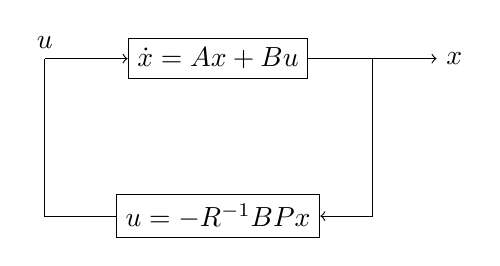
\begin{tikzpicture}[auto,node distance=2cm]
    \tikzstyle{block} = [draw,rectangle]
    \node [block] (dx) {$\dot x = Ax+Bu$};
    \node [right of=dx,node distance=3cm] (x) {$x$};
    \node [block,below of=dx] (u) {$u=-R^{-1}B\trans Px$};
    \node [left of=dx,inner sep=0pt,minimum size=0pt,node distance=2.2cm] (u2) {};
    \node [above] at (u2) {$u$};
    \draw [->] (dx) -- coordinate (x2) (x);
    \draw [->] (x2) |- (u);
    \draw [->] (u) -| (u2) -- (dx);
  \end{tikzpicture}
\end{center}
The closed-loop dynamics are
\begin{gather}
  \dot x = Ax - BR^{-1}B\trans Px = \underbrace{(A-BR^{-1}B\trans P)}_{A_\text{CL}} x
\end{gather}
The ``optimal'' closed-loop eigenvalues (poles) are $\mathop\text{eig}(A-BR^{-1}B\trans P)=-1,-2$. In Matlab, \texttt{K=place(A,B,[-1 -2])=[2 3]}, which are the same.

In Matlab, the ARE is solved by \texttt{P=are(A,B*R\^{}-1*B',Q)}.

\subsection{Linear Quadratic Regulation (LQR)}
Now we have an ``output'', a part of the state we care about given by
\begin{gather}
  y=Cx, \quad y\in\R^m\ (m\le n).
\end{gather}
We want to drive $y\to0$.
\begin{align}
  \min_u {} & \int_0^\infty (y\trans Qy + u\trans Ru) \dif t \\
  \text{s.t. } & \dot x = Ax + Bu \\
            & y = Cx,
\end{align}
where $x\in\R^n,u\in\R^p,y\in\R^m$, $Q\in\R^{m\times m}\succ 0$, and $R\in\R^{p\times p}\succ 0$. We still need $(A,B)$ to be CC and $(A,\sqrt{Q}C)$ to be CO. Typically, $Q=\mathrm{I}$, so $(A,C)$ needs to be CO.

To solve this, we turn it into a LQ problem:
\begin{gather}
  \min_u \int_0^\infty (u\trans Ru + x\trans C\trans Q Cx)\dif t
\end{gather}
The optimal control is $u=-R^{-1}B\trans Px$, where $P=P\trans\succ0$ uniquely solves
\begin{gather}
  A\trans P + PA + C\trans QC - PBR^{-1}B\trans P = 0.
\end{gather}

But what if $y$ is not just an ``output'' but the actual measured output of the system? We can no longer directly compute the control since we don't know $x$. The solution is to estimate $\hat x$ from $y$ and use $\hat x$ instead (observer design). The following figure shows an Luenberger observer.

\begin{center}
  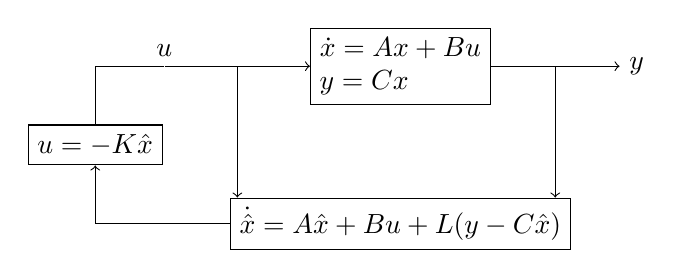
\begin{tikzpicture}[auto,node distance=3cm]
    \tikzstyle{block} = [draw,rectangle]
    \node [block,align=left] (sys) {$\dot x=Ax+Bu$ \\ $y=Cx$};
    \node [right of=sys] (y) {$y$};
    \node [left of=sys,minimum size=0pt,inner sep=0pt] (u) {};
    \node [above] at (u) {$u$};
    \node [block,below of=sys,node distance=2cm] (L) {$\dot{\hat x}=A\hat x+Bu+L(y-C\hat x)$};
    \path (sys.center) -- (L.center) node[pos=0.5] (z) {};
    \node [block,left of=z,node distance=4cm] (control) {$u=-K\hat x$};

    \draw [->] (sys) -- node [pos=0.5] (y2) {} (y);
    \draw [->] (u) -- node [pos=0.5] (u2) {} (sys);
    \draw [->] (y2) -- (y2|-L.north);
    \draw [->] (u2) -- (u2|-L.north);
    \draw [->] (L) -| (control);
    \draw (control) |- (u);
  \end{tikzpicture}
\end{center}
Here, pole placement can be used to place the eigenvalues of $A-LC$ larger than those of the closed-loop system so the observer $\hat x$ converges quickly to the actual $x$.

% 2017/04/13
\section[Connections Between Machine Learning and Optimal Control]{Connections Between Machine Learning and Optimal Control\footnote{Not on final.}}

Recall the discrete-time derivation of Bellman's equation. The system was
\begin{gather}
  x_{k+1} = F(x_k,u_k)
\end{gather}
with cost $c(x_k,u_k)$ for doing $u_k$ at $x_k$. Using $u=u_0,\dots,u_{N-1}$ from $x_0$, the total cost was
\begin{gather}
  V_N^u (x_0) = \sum_{k=0}^{N-1} c(x_k,u_k) + \Theta(x_N).
\end{gather}
Bellman's equation for the optimal cost-to-go is
\begin{align}
  & V_k^* (x) = \min_u \Big\{ c(x,u) + V_{k-1}^* \big( F(x,u) \big) \Big\} \\
  & V_0^* (x) = \Theta(x),
\end{align}
for $k=1,\dots,N$. If we do an infinite-horizon version instead, we would get a \emph{policy} $u = \Pi(x)$, where the control action depends solely on the state and not time. The infinite-horizon cost is
\begin{gather}
  V^\Pi (x) = \sum_{k=0}^\infty c(x_k,\Pi(x_k)) \gamma^k,
\end{gather}
where $\gamma\in(0,1)$ is the discount. The discount ensures the cost converges. Note there is no step count in the notation $V^\Pi$ and no terminal cost. Bellman's equation for the infinite-horizon case is
\begin{gather}
  V^* (x) = \min_u \left\{ c(x,u) + \sum_{k=1}^\infty \gamma^k c\big(x_k,\Pi^*(x_k)\big) \right\}.
\end{gather}
Note that
\begin{align}
  \sum_{k=1}^\infty \gamma^k c\big(x_k,\Pi^*(x_k)\big) &= \gamma \sum_{k=0}^\infty \gamma^k c\big(x_{k+1},\Pi^*(x_{k+1})\big) \\
                                                       &= \gamma \sum_{k=0}^\infty \gamma^k c \Big( F\big(x_k,\Pi^*(x_k)\big), \Pi^*\big(F(x_k,\Pi^*(x_k))\big) \Big) \\
  &= \gamma V^*\big(F(x_0,\Pi^*(x_0)\big)
\end{align}
Then, Bellman's infinite horizon equation is
\begin{gather}
  V^*(x) = \min_u \Big\{ c(x,u) + \gamma V^*\big(F(x,u)\big) \Big\}.
\end{gather}

Let's assume we magically had $V^*(x)$. Then
\begin{gather}
  \Pi^*(x) = \arg\min_u \Big\{ c(x,u) + \gamma V^*\big(F(x,u)\big) \Big\}.
\end{gather}
This works only if we somehow also know $c(x,u)$ and $F(x,u)$ for all $x,u$. The problem is we may not know $c$ and $F$ so we cannot evaluate $\arg\min\{\cdot\}$ even if we knew $V^*(x)\ \forall x$.

What if we were instead given (using magic)
\begin{gather}
  W^*(x,u) = c(x,u) + \gamma \min_v W^*\big(F(x,u),v\big).
\end{gather}
We can rewrite this as
\begin{enumerate}
\item $\min_u W^*(x,u)=V^*(x)$
\item $\Pi^*(x) = \arg\min_u W^*(x,u)$
\end{enumerate}
Note that this is just Bellman's equation. So knowing $W^*(x,u)\ \forall x,u$ (do not need to know $c,F$) is enough for us to know $\Pi^*(x)$! Instead of using magic, we could instead
\begin{enumerate}[nosep]
\item use optimal control (last few weeks)
\item move around in the ``world'', ``experiencing'' the costs as they show up; this is known as \emph{reinforcement learning}
\end{enumerate}

\subsection{Reinforcement Learning}
The idea is to move around (randomly) and build up the values in the Q-table. This is a form of reinforcement learning known as Q-learning.

Let's assume (for now) that $X$ ($x\in X$) and $U$ ($u\in U$) are both finite. Let's call $W^*(x,u)=Q(x,u)$.

\begin{algorithm}[H]
  \caption{Q-learning}
  \begin{algorithmic}
    \State $Q_0(x,u)=q_0\ \forall x,u$
    \State $k=0$
    \Repeat
    \State Pick $(x,u)$ ``randomly'' and update the Q-table through

    \hspace{0.5cm} $ Q_k(x,u) = Q_{k-1}(x,u) + \alpha_k \left[ c(x,u) + \gamma \min_v \Big\{ Q_{k-1} \big(F(x,u),v\big) - Q_{k-1}(x,u) \Big\} \right] $

    \State $k=k+1$
    \Until ``done''
  \end{algorithmic}
\end{algorithm}

\noindent
Note:
\begin{enumerate}[nosep]
\item $c(x,u)$ and $F(x,u)$ are ``experienced'', i.e.\ there is no need to know these in advance
\item $\alpha_k$ is the ``learning rate'' and ``needs'' to satisfy
  \begin{gather}
    \sum \alpha_k^2 < \infty, \qquad \sum \alpha_k = \infty
  \end{gather}
\item If all $(x,u)$ pairs are visited infinitely many times, then $Q_k(x,u)\to Q(x,u)\ \forall x,u$ as $k\to\infty$.
\end{enumerate}

\medskip\noindent
A extension (even for non-finite $X,U$) is to choose a ``fatter'' basis function instead of points. A basis function should have compact support. Examples include sigmoids, wavelets, B-splines, and kernels.

How many basis functions? How to update their amplitudes from the data?

Matlab example \texttt{qlearn} on T-Square.

%%% Local Variables:
%%% mode: latex
%%% TeX-master: "../notes"
%%% End: